\begin{figure*}[t]\centering
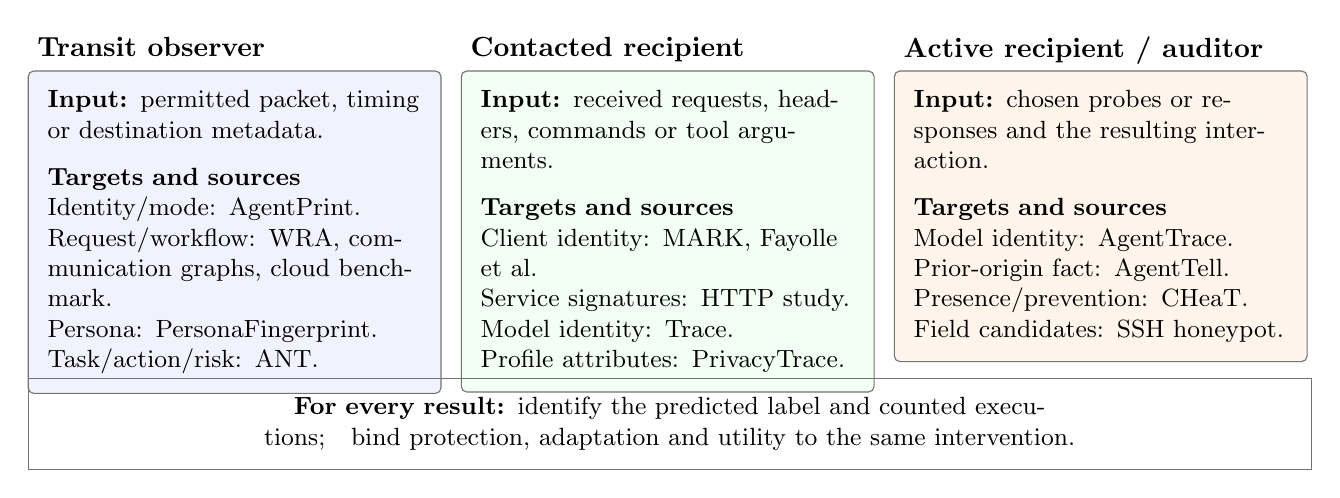
\begin{tikzpicture}[x=1cm,y=1cm,font=\small]
\tikzset{panel/.style={draw=black!55,rounded corners=2pt,align=left,text width=4.75cm,inner sep=7pt,anchor=north west}, head/.style={font=\bfseries,align=left,text width=4.7cm,anchor=north west}}
\node[head] at (0,0) {Transit observer};
\node[head] at (5.5,0) {Contacted recipient};
\node[head] at (11,0) {Active recipient / auditor};
\node[panel,fill=blue!5,minimum height=3.45cm] (p) at (0,-.55) {
\textbf{Input:} permitted packet, timing or destination metadata.\par\medskip
\textbf{Targets and sources}\par
Identity/mode: AgentPrint.\par
Request/workflow: WRA, communication graphs, cloud benchmark.\par
Persona: PersonaFingerprint.\par
Task/action/risk: ANT.};
\node[panel,fill=green!5,minimum height=3.45cm] (r) at (5.5,-.55) {
\textbf{Input:} received requests, headers, commands or tool arguments.\par\medskip
\textbf{Targets and sources}\par
Client identity: MARK, Fayolle et al.\par
Service signatures: HTTP study.\par
Model identity: Trace.\par
Profile attributes: PrivacyTrace.};
\node[panel,fill=orange!8,minimum height=3.45cm] (a) at (11,-.55) {
\textbf{Input:} chosen probes or responses and the resulting interaction.\par\medskip
\textbf{Targets and sources}\par
Model identity: AgentTrace.\par
Prior-origin fact: AgentTell.\par
Presence/prevention: CHeaT.\par
Field candidates: SSH honeypot.};
\node[draw=black!55,align=center,text width=15.8cm,inner sep=7pt,anchor=north west] at (0,-4.45) {\textbf{For every result:} identify the predicted label and counted executions;\quad bind protection, adaptation and utility to the same intervention.};
\end{tikzpicture}
\caption{Evidence space by observation rights. The fifteen studies are placed by the mapped settings, not ranked by accuracy or access strength. Some offer richer additional views; Tables~\ref{tab:attack-map}--\ref{tab:attack-recipient} identify those conditions and their metrics. Known-service signatures and field candidates are descriptive endpoints, not held-out recognition rates.}\label{fig:field-space}
\end{figure*}
